% ===================================================================
% Week 02 -- Dynamics and Coding in the Brain (HUJI 769001)
% Lecture 2: the autapse with a linear activation function, fixed points
% and their stability.
% Reference: Loewenstein, Mongillo, Landau & Fox, The Dynamics of Computation in
% Neuronal Networks (../tcns_book-88.pdf), sec. 2.3.1 (linear part), App. 2.A.1.
% Build: pdflatex -interaction=nonstopmode week02.tex  (twice)
% ===================================================================
% ===================================================================
% Preamble for the Dynamics and Coding in the Brain weekly notes (copy of the shared
% lecture-notes preamble, kept here so this folder builds on its own).
% ===================================================================
\documentclass[11pt,a4paper]{article}

% ---------- encoding & fonts ----------
\usepackage[T1]{fontenc}
\usepackage[utf8]{inputenc}
\usepackage{lmodern}
\renewcommand{\familydefault}{\rmdefault}
\usepackage{microtype}

% ---------- layout ----------
\usepackage[a4paper,margin=2.3cm,top=2.4cm,bottom=2.6cm,headsep=0.9cm]{geometry}
\setlength{\parindent}{0pt}
\setlength{\parskip}{0.55em}
\usepackage{needspace}
\usepackage{multicol}
\usepackage[shortlabels]{enumitem}
\usepackage{array,booktabs,colortbl,tabularx}
\newcolumntype{L}[1]{>{\raggedright\arraybackslash}p{#1}}

% ---------- maths ----------
\usepackage{amsmath,amssymb,mathtools}

% ---------- colours ----------
\usepackage[dvipsnames]{xcolor}
\definecolor{paper}{HTML}{EFE9DA}
\definecolor{surface}{HTML}{FDFBF4}
\definecolor{surface2}{HTML}{F1EBDB}
\definecolor{ink}{HTML}{221C35}
\definecolor{muted}{HTML}{6E6883}
\definecolor{border}{HTML}{4B3C8E}
\definecolor{shadowcol}{HTML}{2E2552}
\definecolor{pgreen}{HTML}{1D6A3B}
\definecolor{ppink}{HTML}{D0307A}
\definecolor{pgold}{HTML}{8C5C0B}
\definecolor{pcyan}{HTML}{2B5FA8}
\pagecolor{paper}
\color{ink}

% ---------- graphics ----------
\usepackage{tikz}
\usetikzlibrary{positioning,arrows.meta,calc,shapes.geometric,shapes.misc,decorations.pathreplacing,patterns,fit,backgrounds}
\usepackage{pgfplots}
\pgfplotsset{compat=1.18}
\tikzset{
  lbl/.style={font=\footnotesize,text=ink,inner sep=1pt},
  blk/.style={draw=ink,line width=1pt,fill=surface,font=\sffamily\scriptsize\bfseries,align=center,minimum height=0.85cm,inner sep=4pt},
  arr/.style={-{Stealth},line width=1.1pt,ink},
  dot/.style={circle,fill=ink,inner sep=1.4pt},
  plbl/.style={font=\ttfamily\scriptsize,text=muted,inner sep=1pt},
  >={Stealth[length=2.6mm]}
}

% ---------- inline semantic markup ----------
\newcommand{\term}[1]{\textcolor{pgreen}{#1}}   % newly defined term
\newcommand{\key}[1]{\textcolor{pcyan}{#1}}     % key word / unit
\newcommand{\hl}[1]{\textcolor{ppink}{#1}}      % the thing to remember
\newcommand{\thd}[1]{{\color{surface}\sffamily\bfseries\footnotesize #1}} % table header cell
\newcommand{\src}[1]{{\ttfamily\scriptsize\textcolor{muted}{[#1]}}}

% ---------- boxes ----------
\usepackage[most]{tcolorbox}
\tcbset{
  notebase/.style={
    enhanced jigsaw, breakable, sharp corners,
    colback=surface, colframe=border, boxrule=1.1pt,
    left=6pt,right=6pt,top=5pt,bottom=5pt,
    before skip=1.1em, after skip=1.1em,
    shadow={1.4mm}{-1.4mm}{0mm}{fill=shadowcol},
    fonttitle=\ttfamily\scriptsize,
    attach boxed title to top left={xshift=3mm,yshift*=-2.4mm},
    boxed title style={sharp corners,boxrule=0.9pt,colframe=surface,
      left=4pt,right=4pt,top=2.5pt,bottom=2.5pt,
      shadow={0.8mm}{-0.8mm}{0mm}{fill=shadowcol}},
    parbox=false,
    before upper={\setlength{\parskip}{0.45em}},
  }
}
\newcommand{\boxtitle}[2]{\if\relax\detokenize{#2}\relax #1\else #1 \textperiodcentered\ \MakeUppercase{#2}\fi}
\newcommand{\boxtitleonly}[2]{\if\relax\detokenize{#2}\relax #1\else \MakeUppercase{#2}\fi}

\newtcolorbox{defn}[1][]{notebase,colbacktitle=pgreen,title={\boxtitle{DEF}{#1}}}
\newtcolorbox{formula}[1][]{notebase,colbacktitle=border,title={\boxtitleonly{FORMULA}{#1}}}
\newtcolorbox{intuition}[1][]{notebase,colbacktitle=ppink,title={\boxtitleonly{KEY IDEA}{#1}}}
\newtcolorbox{example}[1][]{notebase,colbacktitle=pcyan,title={\boxtitle{EXAMPLE}{#1}}}
\newtcolorbox{pitfall}[1][]{notebase,colbacktitle=pgold,title={\boxtitle{PITFALL}{#1}}}
\newtcolorbox{plainbox}{notebase}

% lists inside notes
\setlist[itemize]{label={\textcolor{pgreen}{\scriptsize$\blacksquare$}},leftmargin=1.3em,itemsep=0.25em,topsep=0.3em}
\setlist[enumerate]{label={\textcolor{pgreen}{\ttfamily\arabic*.}},leftmargin=1.6em,itemsep=0.3em,topsep=0.3em}

% ---------- headings ----------
\usepackage{titlesec}
\newcommand{\twodigit}[1]{\ifnum#1<10 0\fi\number#1}
\titleformat{\section}[display]
  {\sffamily\bfseries\fontsize{20}{24}\selectfont\color{pgold}}
  {\ttfamily\small\mdseries\color{pgreen}SECTION \twodigit{\value{section}}}
  {8pt}{}[\vspace{4pt}{\color{border}\titlerule[1.4pt]}]
\titlespacing*{\section}{0pt}{1.6em}{1.0em}
\titleformat{\subsection}
  {\ttfamily\large\color{pcyan}}{>\,\thesubsection}{0.6em}{}
\titlespacing*{\subsection}{0pt}{1.3em}{0.5em}
\titleformat{\subsubsection}
  {\sffamily\bfseries\color{border}}{\thesubsubsection}{0.6em}{}
\titlespacing*{\subsubsection}{0pt}{1.0em}{0.3em}

% ---------- running header / footer ----------
\usepackage{fancyhdr}
\newcommand{\headleft}{}
\newcommand{\headright}{}
\pagestyle{fancy}
\fancyhf{}
\renewcommand{\headrulewidth}{0pt}
\fancyhead[L]{\ttfamily\scriptsize\textcolor{muted}{\headleft}}
\fancyhead[R]{\ttfamily\scriptsize\textcolor{muted}{\headright}}
\fancyfoot[C]{\tikz{\node[draw=border,line width=1pt,fill=surface,inner sep=2.5pt,font=\sffamily\footnotesize] (p) {\thepage};
  \draw[shadowcol,line width=1.6pt] ([yshift=-2pt]p.south west)--([yshift=-2pt]p.south east);}}
\fancypagestyle{plain}{\fancyhf{}\renewcommand{\headrulewidth}{0pt}\fancyfoot[C]{\tikz{\node[draw=border,line width=1pt,fill=surface,inner sep=2.5pt,font=\sffamily\footnotesize] (p) {\thepage};
  \draw[shadowcol,line width=1.6pt] ([yshift=-2pt]p.south west)--([yshift=-2pt]p.south east);}}}

% ---------- links ----------
\usepackage[hidelinks]{hyperref}

\renewcommand{\headleft}{769001 \textperiodcentered\ WEEK 02}
\renewcommand{\headright}{DYNAMICS AND CODING IN THE BRAIN}

\newcommand{\figcap}[1]{\par\smallskip{\small\color{muted}#1}\par}
\newcommand{\hext}{h^{\text{ext}}}
\newcommand{\dr}{\delta r}

\begin{document}

% ---------------- title block ----------------
{\ttfamily\small\color{pgreen}HUJI \textperiodcentered\ 769001 \textperiodcentered\ DYNAMICS AND CODING IN THE BRAIN}\par\vspace{6pt}
{\sffamily\bfseries\fontsize{30}{34}\selectfont\color{pgold}Week 02}\par\vspace{4pt}
{\sffamily\bfseries\Large\color{pgold}The Autapse: Fixed Points and Stability}\par\vspace{4pt}
{\ttfamily\small\color{pcyan}autapse \textperiodcentered\ linear activation \textperiodcentered\ fixed point \textperiodcentered\ perturbation \textperiodcentered\ stability \textperiodcentered\ vector field}\par
\vspace{0.8em}

{\ttfamily\small\color{pgreen}CONTENTS}
\begin{multicols}{2}\footnotesize\setlength{\parskip}{0pt}
\setcounter{tocdepth}{1}
\makeatletter\@starttoc{toc}\makeatother
\end{multicols}

\section{Where we are}

Week 1 ended with the rate model of a network of $N$ neurons \src{LMLF eq.\ 2.8--2.9}:
\[ \tau\dot r_i = -r_i + g(h_i),\qquad h_i = \sum_{j=1}^N J_{ij}r_j + \hext_i. \]
\begin{itemize}
  \item $r_i$ is the firing rate of neuron $i$; $\tau$ is its time constant ($\sim$10\,ms).
  \item $h_i$ is its total input: what it hears from the other neurons ($J_{ij}r_j$, synapse \emph{from} $j$ \emph{to} $i$) plus external input $\hext_i$.
  \item $g$ is the activation function: it turns input into a rate.
\end{itemize}

\begin{intuition}[The plan for this week]
Before analysing big networks, study the \hl{smallest possible network: one neuron}. If it talks to itself, it already has
\emph{feedback}, and feedback is what makes networks interesting. This week we use it to introduce two tools we will use all course long:
\textbf{fixed points} and their \textbf{stability}.
\end{intuition}

\section{The autapse}

\begin{defn}[Autapse]
An \term{autapse} is a synapse that a neuron makes \hl{onto itself}: its axon connects back to its own dendrites. A neuron with an autapse is
\emph{the simplest possible network}: one neuron, one connection, of strength $J$ \src{LMLF 2.3.1}.
\end{defn}

\begin{center}
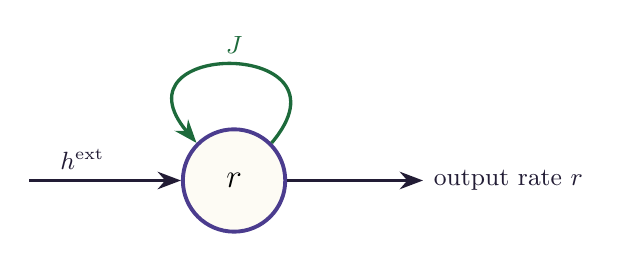
\begin{tikzpicture}[>=Stealth]
  \node[circle,draw=border,line width=1.4pt,fill=surface,minimum size=1.3cm,font=\large] (n) at (0,0) {$r$};
  \draw[->,line width=1.2pt,ink] (-2.6,0) -- (n.west) node[pos=0.35,above,font=\small]{$\hext$};
  \draw[->,line width=1.2pt,pgreen] (n.north east) .. controls (1.6,1.8) and (-1.6,1.8) .. (n.north west)
        node[pos=0.5,above,font=\small]{$J$};
  \draw[->,line width=1.2pt,ink] (n.east) -- (2.4,0) node[right,font=\small]{output rate $r$};
\end{tikzpicture}
\figcap{The autapse (after \src{LMLF Fig.\ 2.6}). The neuron receives an external input $\hext$, and its own output $r$ comes back to it through the synapse of strength $J$.}
\end{center}

With a single neuron, the network equations lose their indices \src{LMLF eq.\ 2.11--2.12}:
\begin{formula}[Autapse dynamics]
\[ \tau\dot r = -r + g(h),\qquad h = Jr + \hext. \]
\end{formula}

\begin{defn}[Excitatory autapse]
We focus on \term{excitatory} autapses, $J>0$: the more the neuron fires, the more input it gives itself. This is \term{positive feedback}.
\end{defn}

\begin{example}[One input value, two sources]
$J=0.5$, $\hext=1$, current rate $r=4$: total input $h = 0.5\cdot4+1 = 3$. Two of the three units of input come from the neuron itself.
\end{example}

\section{The linear autapse}

\begin{defn}[Linear activation function]
The \term{linear} (identity) activation function is $g(h)=h$: the rate equals the input, with no threshold and no saturation \src{LMLF eq.\ 2.4}.
\end{defn}

\begin{pitfall}[Why linear is a simplification]
A real neuron cannot fire at a negative rate, and it cannot fire faster than a few hundred Hz. The linear $g$ ignores both limits. We use it
because the resulting equation is linear, so we can solve it and understand it completely. It is a good approximation when the rate changes only a little.
\end{pitfall}

With $g(h)=h$ the autapse equation becomes
\[ \tau\dot r = -r + Jr + \hext \qquad\Longrightarrow\qquad \boxed{\ \tau\dot r = -(1-J)\,r + \hext\ } \]

\begin{intuition}[Two forces on $r$]
\begin{itemize}
  \item $-r$: the \term{leak}. Left alone, the rate decays back to zero (Week 1).
  \item $+Jr$: the \term{feedback}. The neuron excites itself in proportion to its own rate.
\end{itemize}
The whole story of this week is the \hl{contest between leak and feedback}: who wins depends on whether $J<1$ or $J>1$.
\end{intuition}

This is exactly the equation $\dot n = an + I$ from the Week 1 bonus hour, with $a = -(1-J)/\tau$ and constant input $I=\hext/\tau$. We could solve it right away
(we do so in \S\ref{sec:solution}). But first we introduce an approach that works \emph{even when the equation cannot be solved}: look for the fixed points and ask whether they are stable.

\section{Fixed points}

\begin{defn}[Fixed point]
A \term{fixed point} $r^*$ is a value of $r$ where the dynamics stand still: \hl{$\dot r = 0$}. If the system starts exactly at $r^*$, it stays there forever \src{LMLF 2.3.1}.
\end{defn}

\textbf{Finding it.} Set the right-hand side to zero:
\[ 0 = -(1-J)\,r^* + \hext \qquad\Longrightarrow\qquad \boxed{\ r^* = \frac{\hext}{1-J}\ }\qquad (J\neq1). \]

\begin{example}[Fixed points for $\hext = 1$]
\begin{center}
\renewcommand{\arraystretch}{1.25}
\begin{tabular}{>{\columncolor{border}}c c l}
\thd{$J$} & \cellcolor{border}\thd{$r^*=1/(1-J)$} & \cellcolor{border}\thd{COMMENT}\\
\rowcolor{surface} \cellcolor{border}\color{surface}$0$ & $1$ & no feedback: the rate just copies the input\\
\rowcolor{surface2} \cellcolor{border}\color{surface}$0.5$ & $2$ & feedback doubles the response\\
\rowcolor{surface} \cellcolor{border}\color{surface}$0.9$ & $10$ & strong feedback: ten times the input\\
\rowcolor{surface2} \cellcolor{border}\color{surface}$0.99$ & $100$ & close to $J=1$ the fixed point runs off\\
\rowcolor{surface} \cellcolor{border}\color{surface}$1.5$ & $-2$ & negative! (see below)\\
\end{tabular}
\end{center}
\end{example}

\begin{intuition}[Feedback amplifies]
For $0<J<1$, $r^* = \hext/(1-J) > \hext$: the autapse \hl{amplifies its input by the factor $1/(1-J)$}.
Why: the input raises $r$, which raises the feedback $Jr$, which raises $r$ further, and so on. The extra contributions add up to
$\hext(1+J+J^2+\dots) = \hext/(1-J)$, a geometric series that converges only if $J<1$.
\end{intuition}

\begin{pitfall}[A fixed point is not automatically where the system goes]
For $J=1.5$ the formula gives $r^*=-2$. It is a perfectly valid solution of $\dot r=0$, but (as we will see) the system runs \emph{away} from it.
Also, a negative rate shows that the linear model has left the range where it describes a real neuron. Finding a fixed point is only half the job; the other half is its stability.
\end{pitfall}

\begin{pitfall}[The border case $J=1$]
For $J=1$ the leak and the feedback cancel exactly: $\tau\dot r = \hext$. If $\hext\neq0$ there is \emph{no} fixed point ($r$ grows or shrinks steadily).
If $\hext=0$ then $\dot r=0$ everywhere: \emph{every} value of $r$ is a fixed point. The book returns to this special case later (\S4.2); this week we assume $J\neq1$.
\end{pitfall}

\section{Stability}

\subsection{The idea}

\begin{defn}[Stable and unstable fixed points]
Start the system \emph{near} $r^*$ instead of exactly on it.
\begin{itemize}
  \item If the dynamics bring $r$ \hl{ever closer} to $r^*$, the fixed point is \term{stable}.
  \item If the dynamics \hl{push $r$ away} from $r^*$, the fixed point is \term{unstable}.
\end{itemize}
\end{defn}

\begin{center}
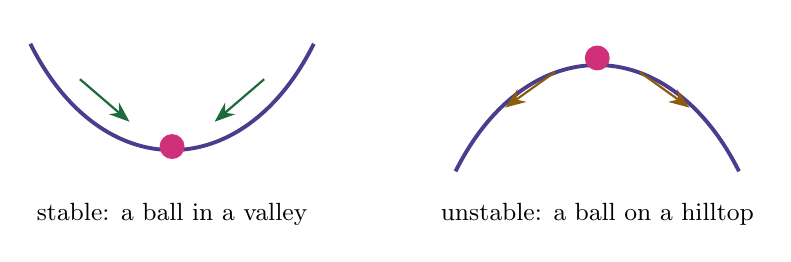
\begin{tikzpicture}[scale=0.9]
  \begin{scope}
    \draw[line width=1.4pt,border] (-2,1.4) .. controls (-1,-0.6) and (1,-0.6) .. (2,1.4);
    \fill[ppink] (0,-0.05) circle (5pt);
    \draw[->,thick,pgreen] (-1.3,0.9)--(-0.6,0.3);
    \draw[->,thick,pgreen] (1.3,0.9)--(0.6,0.3);
    \node[font=\small] at (0,-1){stable: a ball in a valley};
  \end{scope}
  \begin{scope}[xshift=6cm]
    \draw[line width=1.4pt,border] (-2,-0.4) .. controls (-1,1.6) and (1,1.6) .. (2,-0.4);
    \fill[ppink] (0,1.2) circle (5pt);
    \draw[->,thick,pgold] (-0.6,1.0)--(-1.3,0.5);
    \draw[->,thick,pgold] (0.6,1.0)--(1.3,0.5);
    \node[font=\small] at (0,-1){unstable: a ball on a hilltop};
  \end{scope}
\end{tikzpicture}
\figcap{Both balls are at rest (fixed points). A small nudge brings the left ball back but sends the right one rolling away.}
\end{center}

\begin{intuition}[Why stability matters]
In the real brain the rate is never exactly at $r^*$: there is always noise. An unstable fixed point is never seen in practice, because the
tiniest disturbance grows. Only \hl{stable fixed points describe states the network actually sits in}.
\end{intuition}

\subsection{Perturbation analysis, step by step}

To decide stability, follow a small deviation from the fixed point \src{LMLF eq.\ 2.14--2.15}.

\begin{defn}[Perturbation]
The \term{perturbation} is the distance from the fixed point: $\dr(t) = r(t)-r^*$. Equivalently $r = r^*+\dr$.
\end{defn}

\begin{enumerate}
  \item \textbf{Substitute} $r = r^*+\dr$ into $\tau\dot r = -r+Jr+\hext$:
        \[ \tau\frac{d}{dt}(r^*+\dr) = -(r^*+\dr) + J(r^*+\dr) + \hext. \]
  \item \textbf{$r^*$ is a number, not a function of time}, so $\frac{d}{dt}r^* = 0$ and the left side is $\tau\,\dot{\dr}$.
  \item \textbf{Regroup the right side} into the part with $r^*$ and the part with $\dr$:
        \[ \tau\,\dot{\dr} = \underbrace{\big(-r^*+Jr^*+\hext\big)}_{=\,0\ \text{(definition of } r^*)} + \big(-\dr + J\dr\big). \]
  \item \textbf{The first bracket vanishes} because $r^*$ is a fixed point. What remains is
        \[ \boxed{\ \tau\,\dot{\dr} = -(1-J)\,\dr\ } \]
\end{enumerate}

\begin{intuition}[What happened]
The external input $\hext$ has disappeared. It only decides \emph{where} the fixed point is; whether the fixed point is stable depends only on $J$.
\end{intuition}

\subsection{Reading off stability from the sign}

\textbf{Case $J<1$}, so $1-J>0$:
\begin{itemize}
  \item if $\dr>0$ (rate above the fixed point) then $\dot{\dr}<0$: it comes down;
  \item if $\dr<0$ (rate below) then $\dot{\dr}>0$: it goes up.
\end{itemize}
Either way the perturbation shrinks. \hl{The fixed point is stable.}

\textbf{Case $J>1$}, so $1-J<0$: now $\dot{\dr}$ has the \emph{same} sign as $\dr$. Above the fixed point the rate rises further; below it, it falls further.
\hl{The fixed point is unstable.}

\begin{formula}[Stability of the linear autapse]
\[ J<1\ \Rightarrow\ \text{stable}\qquad\qquad J>1\ \Rightarrow\ \text{unstable} \]
$J=1$ is the border between two qualitatively different behaviours.
\end{formula}

\begin{intuition}[Leak vs.\ feedback again]
$J<1$: when the rate goes up by $\dr$, the leak pulls it down by $\dr$ but the feedback pushes it up only by $J\dr<\dr$. Leak wins, the deviation dies.
$J>1$: the feedback push $J\dr$ beats the leak, the deviation feeds itself.
\end{intuition}

\subsection{How fast? Solving for $\dr(t)$}

$\tau\dot{\dr} = -(1-J)\dr$ is the Week 1 equation $\dot n = an$ with $a = -(1-J)/\tau$, so \src{LMLF eq.\ 2.16}
\begin{formula}[Perturbation over time]
\[ \dr(t) = \dr(0)\,e^{-(1-J)t/\tau}. \]
\end{formula}
\begin{itemize}
  \item $J<1$: exponential \textbf{decay} to $0$, i.e.\ $r(t)\to r^*$.
  \item $J>1$: exponential \textbf{growth}; $r$ diverges to $+\infty$ or $-\infty$, depending on the sign of $\dr(0)$.
\end{itemize}

\begin{example}[How long a perturbation lasts, $\tau = 10$\,ms]
The perturbation shrinks (or grows) by a factor $e$ every $\tau/|1-J|$:
\begin{center}
\renewcommand{\arraystretch}{1.25}
\begin{tabular}{>{\columncolor{border}}c c c}
\thd{$J$} & \cellcolor{border}\thd{$\tau/|1-J|$} & \cellcolor{border}\thd{BEHAVIOUR}\\
\rowcolor{surface} \cellcolor{border}\color{surface}$0$ & 10\,ms & decays (just the leak)\\
\rowcolor{surface2} \cellcolor{border}\color{surface}$0.5$ & 20\,ms & decays, twice as slowly\\
\rowcolor{surface} \cellcolor{border}\color{surface}$0.9$ & 100\,ms & decays, ten times as slowly\\
\rowcolor{surface2} \cellcolor{border}\color{surface}$1.5$ & 20\,ms & grows by $e$ every 20\,ms\\
\end{tabular}
\end{center}
The closer $J$ is to $1$, the \hl{slower} everything happens: stronger feedback lets the neuron hold on to a deviation for much longer than its own $\tau$.
\end{example}

\section{The full solution}\label{sec:solution}

Using the Week 1 result for $\dot n = an + I$ with constant input (or simply $r = r^*+\dr$ with $\dr(t)$ from above):
\begin{formula}[Linear autapse, solved]
\[ r(t) = r^* + \big(r(0)-r^*\big)\,e^{-(1-J)t/\tau},\qquad r^*=\frac{\hext}{1-J}. \]
\end{formula}

\textbf{Check.} At $t=0$: $r(0) = r^* + r(0) - r^* = r(0)$ \checkmark. Differentiate:
$\tau\dot r = -(1-J)(r(0)-r^*)e^{-(1-J)t/\tau} = -(1-J)(r-r^*) = -(1-J)r + (1-J)r^* = -(1-J)r + \hext$. \checkmark

\begin{example}[Starting from silence, $r(0)=0$, $\hext=1$, $\tau=10$\,ms]
\begin{center}
\renewcommand{\arraystretch}{1.2}
\begin{tabular}{c|cccccc}
$t$ (ms) & 0 & 10 & 20 & 40 & 60 & 100\\\hline
$J=0.5$: \ $2(1-e^{-t/20})$ & 0 & 0.79 & 1.26 & 1.73 & 1.90 & 1.99\\
$J=0.9$: \ $10(1-e^{-t/100})$ & 0 & 0.95 & 1.81 & 3.30 & 4.51 & 6.32\\
$J=1.5$: \ $-2+2e^{t/20}$ & 0 & 1.30 & 3.44 & 12.8 & 38.2 & 295\\
\end{tabular}
\end{center}
$J=0.5$ settles at $2$ within $\sim$60\,ms. $J=0.9$ heads for $10$ but needs hundreds of ms. $J=1.5$ starts \emph{above} its fixed point $-2$, so it is pushed further and further up, without limit.
\end{example}

\begin{center}
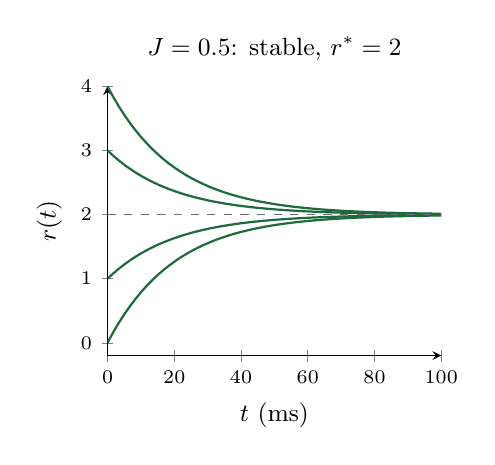
\begin{tikzpicture}
\begin{axis}[width=0.48\linewidth,height=5cm,xmin=0,xmax=100,ymin=-0.2,ymax=4,
  xlabel={$t$ (ms)},ylabel={$r(t)$},axis lines=left,tick label style={font=\scriptsize},label style={font=\small},
  title={\small $J=0.5$: stable, $r^*=2$},title style={font=\small}]
  \foreach \r in {0,1,3,4}{\addplot[pgreen,thick,domain=0:100,samples=60]{2+(\r-2)*exp(-x/20)};}
  \addplot[muted,dashed,domain=0:100]{2};
\end{axis}
\end{tikzpicture}\hfill
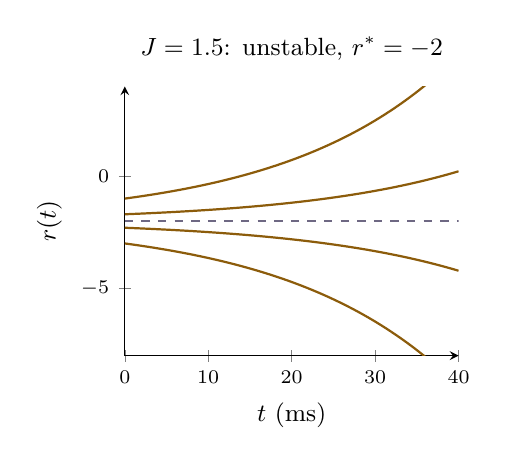
\begin{tikzpicture}
\begin{axis}[width=0.48\linewidth,height=5cm,xmin=0,xmax=40,ymin=-8,ymax=4,
  xlabel={$t$ (ms)},ylabel={$r(t)$},axis lines=left,tick label style={font=\scriptsize},label style={font=\small},
  title={\small $J=1.5$: unstable, $r^*=-2$},title style={font=\small}]
  \foreach \r in {-1,-1.7,-2.3,-3}{\addplot[pgold,thick,domain=0:40,samples=60]{-2+(\r+2)*exp(x/20)};}
  \addplot[muted,dashed,domain=0:40]{-2};
\end{axis}
\end{tikzpicture}
\figcap{$r(t)$ from four starting points ($\tau=10$\,ms, $\hext=1$). Left: every trajectory converges to the dashed fixed point. Right: every
trajectory that does not start exactly on the fixed point is driven away from it.}
\end{center}

\section{The geometric view: the vector field}

We can see stability \emph{without solving anything}, by plotting $\dot r$ as a function of $r$ (the idea from the Week 1 bonus hour).

\begin{defn}[Vector field on a line]
The equation $\tau\dot r = F(r)$ assigns a velocity $\dot r$ to every value of $r$: a \term{vector field} on the line \src{LMLF 2.3.1}.
Draw $\dot r$ against $r$ and put arrows on the $r$-axis: \hl{right where $\dot r>0$, left where $\dot r<0$}. The fixed points are where the graph crosses zero.
\end{defn}

\begin{center}
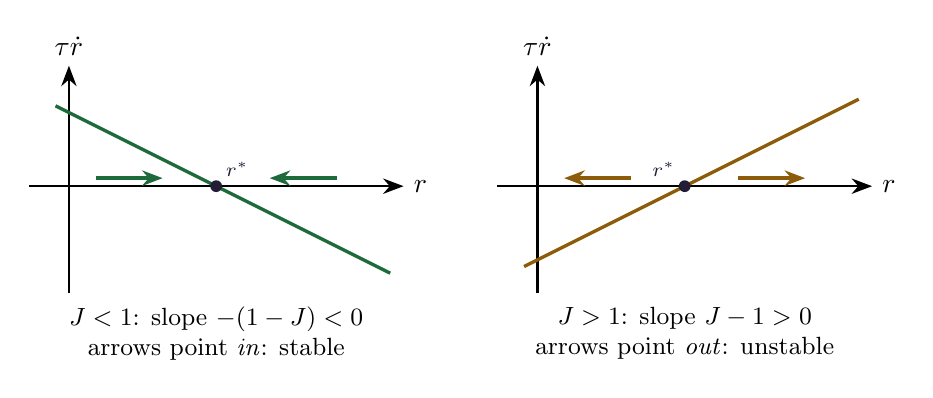
\begin{tikzpicture}[scale=0.85]
  \begin{scope}
    \draw[->,thick] (-2.8,0)--(2.8,0) node[right]{$r$};
    \draw[->,thick] (-2.2,-1.6)--(-2.2,1.8) node[above]{$\tau\dot r$};
    \draw[pgreen,very thick] (-2.4,1.2)--(2.6,-1.3);
    \fill[ink] (0,0) circle (2.5pt) node[above right,font=\scriptsize]{$r^*$};
    \draw[->,very thick,pgreen] (-1.8,0.12)--(-0.8,0.12);
    \draw[->,very thick,pgreen] (1.8,0.12)--(0.8,0.12);
    \node[font=\small,align=center] at (0,-2.2){$J<1$: slope $-(1-J)<0$\\ arrows point \emph{in}: stable};
  \end{scope}
  \begin{scope}[xshift=7cm]
    \draw[->,thick] (-2.8,0)--(2.8,0) node[right]{$r$};
    \draw[->,thick] (-2.2,-1.6)--(-2.2,1.8) node[above]{$\tau\dot r$};
    \draw[pgold,very thick] (-2.4,-1.2)--(2.6,1.3);
    \fill[ink] (0,0) circle (2.5pt) node[above left,font=\scriptsize]{$r^*$};
    \draw[->,very thick,pgold] (-0.8,0.12)--(-1.8,0.12);
    \draw[->,very thick,pgold] (0.8,0.12)--(1.8,0.12);
    \node[font=\small,align=center] at (0,-2.2){$J>1$: slope $J-1>0$\\ arrows point \emph{out}: unstable};
  \end{scope}
\end{tikzpicture}
\figcap{$\tau\dot r = -(1-J)r+\hext$ is a straight line in $r$ that crosses zero at $r^*$. Its slope decides everything.}
\end{center}

\begin{formula}[Stability from the slope]
A fixed point is stable if the graph of $\dot r$ against $r$ crosses zero going \textbf{down} (negative slope),
and unstable if it crosses going \textbf{up} (positive slope). For the linear autapse the slope is $-(1-J)/\tau$: negative exactly when $J<1$.
\end{formula}

\begin{intuition}[Why this is powerful]
This picture needs only the \emph{sign} of $\dot r$ around $r^*$. It works for equations we cannot solve, which will be the usual case once $g$ is not linear.
\end{intuition}

\section{Connection to Week 1: it is the eigenvalue}

In the TA session of Week 1 we saw that $\dot{\vec x} = M\vec x$ converges iff all eigenvalues of $M$ are negative. The perturbation equation
\[ \dot{\dr} = \underbrace{-\frac{1-J}{\tau}}_{\text{a }1\times1\text{ ``matrix''}}\,\dr \]
is the one-dimensional case: its only eigenvalue is $-(1-J)/\tau$, negative exactly when $J<1$. \hl{Stability of a fixed point = the sign of the eigenvalue of the perturbation dynamics.}
For networks of many neurons the same recipe gives a matrix, and Week 1's eigenvalue tools take over.

\section{A limitation of the linear model}

\begin{pitfall}[Divergence is not biology]
For $J>1$ the linear autapse fires at a rate that grows without bound (or goes to $-\infty$). Real neurons \emph{saturate}: their rate cannot exceed a few hundred Hz,
and it cannot go below zero. This is a limitation of the linear $g$, not of the autapse itself. It is the reason the book next replaces $g(h)=h$
by a saturating activation function \src{LMLF 2.3.1}.
\end{pitfall}

\section{Practice problems with full solutions}

\begin{example}[P1: Fixed point and stability]
$\tau\dot r = -r + 0.8r + 3$. Find $r^*$, decide stability, and give $r(t)$ for $r(0)=0$, $\tau=10$\,ms.

\textbf{Solution.} $J=0.8$, $\hext=3$: $r^* = 3/0.2 = 15$. $J<1$, so stable. $r(t) = 15(1-e^{-0.2t/10}) = 15(1-e^{-t/50})$: the time scale is $50$\,ms, five times $\tau$.
\end{example}

\begin{example}[P2: Which $J$ gives a target rate?]
With $\hext=2$, what $J$ makes the stable fixed point $r^*=8$?

\textbf{Solution.} $8 = 2/(1-J)\Rightarrow 1-J = 0.25\Rightarrow J=0.75$. Since $0.75<1$ it is stable. \checkmark
\end{example}

\begin{example}[P3: Perturbation by hand]
$J=1.2$, $\hext=-0.4$, $\tau=10$\,ms. Find $r^*$. The rate starts at $r(0)=2.1$; what is it after $50$\,ms?

\textbf{Solution.} $r^* = -0.4/(1-1.2) = -0.4/(-0.2) = 2$. $J>1$: unstable. $\dr(0)=0.1$, and $\dr(t) = 0.1\,e^{0.2t/10} = 0.1\,e^{t/50}$.
At $t=50$: $\dr = 0.1e\approx0.27$, so $r\approx2.27$. The rate drifts away from $2$, slowly at first and then faster and faster.
\end{example}

\begin{example}[P4: Vector field]
Sketch $\tau\dot r$ against $r$ for $\tau\dot r = -0.5r + 1$ and use it to say what happens from $r(0)=5$.

\textbf{Solution.} A line with slope $-0.5$ crossing zero at $r^*=2$. At $r=5$: $\tau\dot r = -1.5<0$, so $r$ decreases, and it keeps decreasing until it reaches $2$.
The arrows point towards $2$ from both sides: stable.
\end{example}

\begin{example}[P5: The border]
What happens for $J=1$, $\hext=0.5$, $\tau=10$\,ms, $r(0)=0$?

\textbf{Solution.} $\tau\dot r = 0.5$, so $\dot r = 0.05$ per ms: $r(t)=0.05t$, a straight line. There is no fixed point; the rate grows steadily, not exponentially.
\end{example}

\section{Cheat sheet}

\begin{formula}[Week 02 on one page]
\begin{itemize}
  \item \textbf{Autapse}: a neuron's synapse onto itself, strength $J$. $\;\tau\dot r = -r + g(Jr+\hext)$. Excitatory: $J>0$ (positive feedback).
  \item \textbf{Linear} $g(h)=h$: $\;\tau\dot r = -(1-J)r + \hext$. Leak $-r$ vs.\ feedback $+Jr$.
  \item \textbf{Fixed point}: $\dot r=0$. Linear autapse: $r^* = \hext/(1-J)$ ($J\neq1$). For $0<J<1$, an amplification by $1/(1-J)$.
  \item \textbf{Stable}: nearby states return; \textbf{unstable}: nearby states run away. Only stable fixed points are seen in practice.
  \item \textbf{Perturbation}: $\dr = r-r^*$; $\tau\dot{\dr} = -(1-J)\dr$; $\dr(t) = \dr(0)e^{-(1-J)t/\tau}$. $\hext$ drops out.
  \item $J<1$: stable, decay time $\tau/(1-J)$ (slower as $J\to1$). $J>1$: unstable, divergence. $J=1$: border (no fixed point, or a whole line of them).
  \item \textbf{Full solution}: $r(t) = r^* + (r(0)-r^*)e^{-(1-J)t/\tau}$.
  \item \textbf{Vector field}: plot $\dot r$ vs.\ $r$; crossing zero going down = stable, going up = unstable.
  \item Stability = sign of the eigenvalue of the perturbation dynamics (here $-(1-J)/\tau$), as in Week 1.
\end{itemize}
\end{formula}

\end{document}
